\documentclass[12pt]{article}

\usepackage{sbc-template}
\usepackage{listings}
\usepackage{graphicx,url}

\usepackage[english]{babel}   
%\usepackage[latin1]{inputenc}  
\usepackage[utf8]{inputenc}  
% UTF-8 encoding is recommended by ShareLaTex

     
\sloppy

\title{An extension for space-temporal data visualization\\ in TerraView}

\author{Matheus C. Zaglia\inst{1}, Carolina G. Santos\inst{1}, Lúbia
  Vinhas\inst{1}, Gilberto R. Queiroz\inst{1} }


\address{Image Processing Division (DPI)\\ National Institute of Space Research
  (INPE)\\
  Caixa Postal 515 -- 12.245-97 -- São José dos Campos -- SP -- Brazil
  \email{mzaglia@dpi.inpe.br, carolinagalvaosantos@gmail.com}
  \email{\{lubia.vinhas,gilberto.queiroz\}@inpe.br}
}



\begin{document} 

\maketitle

\begin{abstract}
  One of the difficulties presented in some Geographic Information Systems is visualize data based on their timeline, especially when they have fixed locations making it difficult to identify changes from one date to another. Therefore, this work proposes to develop an extension for TerraView using TerraLib capable of satisfying the need to perform data visualization based on time in an easy and intuitive way to GIS users.
\end{abstract}


\section{Introduction}

Geographic Information Systems (GIS) were developed to represent, manage and analyze phenomena that occur in the geographical space, using computational techniques. GIS allow users to perform complex tasks that often integrate data from a variety of sources, building geo-referenced databases, while still enabling the automation of the production of cartographic documents \cite{camara:01}. GIS allow the use of computers as a tool for representing spatially referenced data, solving the problem of how to represent the geographic space, or the real world, as digital information. 

Each day we notice an increase in the volume of spatio-temporal data that are produced by mobile devices and other remote sensors, opening new possibilities to analysis of phenomena that vary over time, allowing the monitoring of objects spatially located in time, as well as improving the resolution of observations. 

As conventional GIS applications are developed for static spatial analysis, we still notice difficulties in modeling systems to represent and perform successful analyzes of temporal phenomena. Currently, there is no consensus on how to represent spatiotemporal information in computational system \cite {karine:15}, so there is not a standard or a complete methodology that includes time in geographical systems. 

Spatio-temporal data are difficult to manipulate because often they are obtained as a long set of individual records of measures, positions associated to an object or a sensor with a time stamp. To manipulate these datasets we need to have specially designed tools, that support the treatment pre-processing and summarization in a more compact representation. 

Currently, enabling the visualization of data based on its timeline is difficult to be done in most conventional GIS applications, especially when they have fixed locations, such as a database that has several records of a single object in different times, but on each date this object can undergo changes in some of its attributes. Example of such tools is 
 \textit{Time Manager} plugin available in the open source QGIS aplication \cite{qgis}. This tool  allows users to animate layers based on their time attributes and the \textit{Traking Analyst} module from ArcGIS \cite{arcgis} where users can add temporal data, visualize then dinamically and handle it as trajectories of objects.

In this work we propose the development of GIS extension that makes it possible to dynamically visualize temporal data in a more simple and intuitive way.

\section{Methods and Materials}

Our extension was developed to the GIS TerraView, an open source project carried on in the  Image Processing Division (DPI) of National Institute for Space Research (INPE). TerraView is based on  \textit{TerraLib} which is an open source geoprocessing library written in C++ language that supports the construction of geographic applications. TerraView has an geographic data display area, and implements several analysis and query funcionalities. It allows the manipulation of vector and raster geographic data, which can be stored relational or geo-relational databases, such as \textit{MySQL} and \textit{PostgreSQL}.

\begin{figure}[ht]
\centering
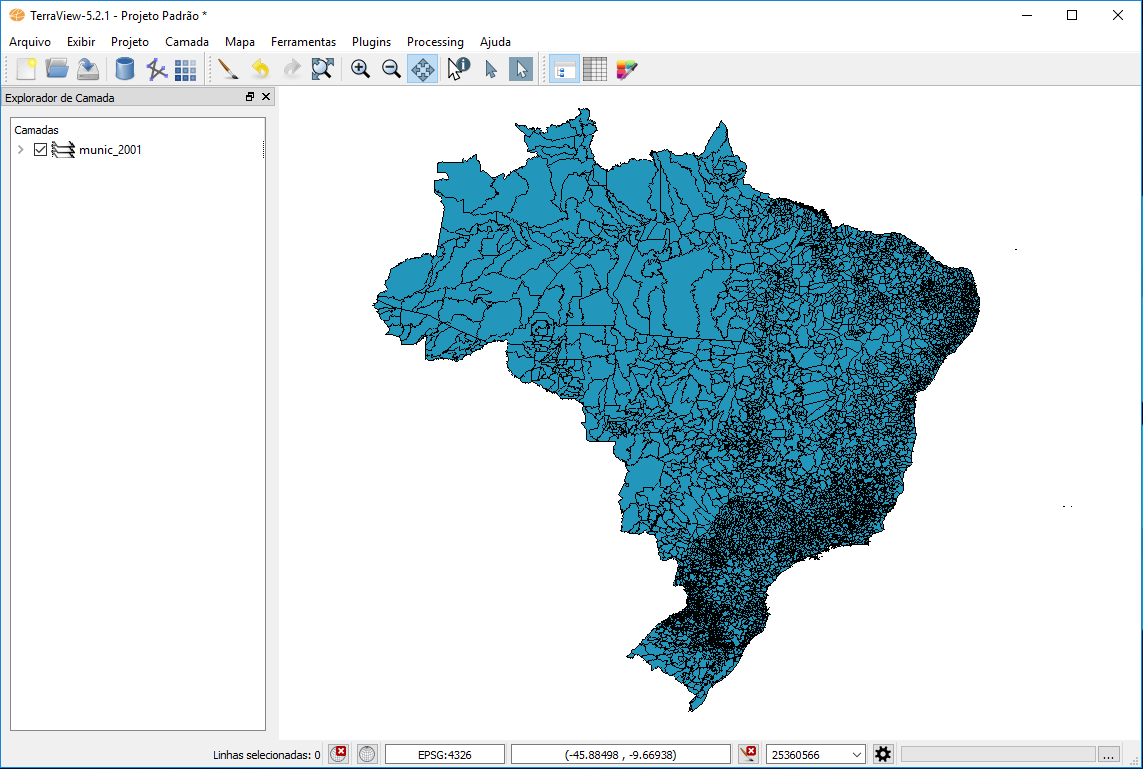
\includegraphics[width=.6\textwidth]{terraview.png}
\caption{TerraView version 5.2.1}
\label{fig:terraviewLayout}
\end{figure}

TerraLib provides the \textit{Spatio-Temporal} module, that implements the types of data and its operations proposed  in the algebra created by \cite{karine:14}. It also allows combination of  different types of  presented in the algebra. The set of data types are summarized in Figure~\ref{fig:exampleKarine}.

\begin{figure}[ht]
\centering
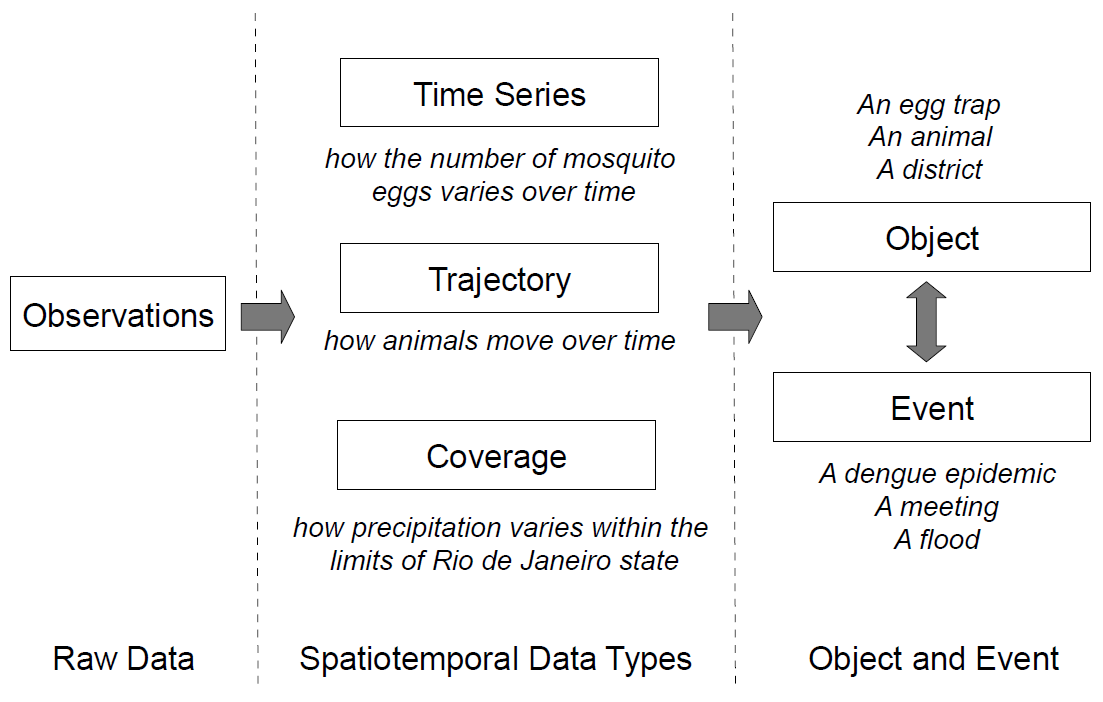
\includegraphics[width=.6\textwidth]{karine-model.png}
\caption{Spatial-temporal data model proposed by Karine}
\label{fig:exampleKarine}
\end{figure}

The \textit{Spatio-Temporal} module also provide a tool with a similar objective to the proposed in this work, to allow the visualization of  complex and large-scale temporal data. In this work we aim at developing a more simple tool to visualize temporal data. All these concepts were implemented in the TerraLib library, in addition to other functionalities that are currently being developed.


The extension was implemented as a TerraLib plugin for version 5.2. It basically consists of layout elements available through the Qt \cite{qt} tool of version 5.4.1, that allows cross-platform development of applications with graphical interfaces. TerraLib's \textit{Data Access} module is responsible for accessing and querying data from different
kinds of sources. It was developed in the C++ programming language using as a development environment Visual Studio 2013 through the Windows 10 operating system. This extension is compatible with all the operating systems that TerraLib supports including Mac and Linux.

The set of data that will be used for the validation of the extension are samples of points distributed throughout the geographic space and samples with fixed location, where their attributes vary over time. The data were obtained through a relational database used by the E-Sensing \cite{esensing} project to perform tests. We also used  shape files  from INPE's fire  detection from satellite data. It is worth mentioning that the extension only needs vector data with temporal attributes.

\section{Development}

This extension will allow from a sample data to view the records of an object according to a timeline in a period determined by the user, making it possible to produce an animation of the object over time. It was called a Time Viewer and built as a plugin of the TerraLib library, where it will be made available using the TerraView application interface to couple the tool's layout.

A new module was created in TerraLib that will be loaded by TerraLib through the \textit{plugins} system. The \textit{Plugin.h} file describes the \textit{te::tv::Plugin} class that inherits the \textit{startup} and \textit{shutdown} methods of class \textit{te::core::Plugin}. In its implementation made in the \textit{Plugin.cpp} file, the startup method is responsible for registering in the TerraView plugins menu an option that creates and displays the extension window and the shutdown method removes previously created pointers.

The extension window has a \textit{combo box} with a list of \textit{layers} that allows the selection of a layer previously added by the user. When selecting a combo item from layers, two other combo boxes are filled with all attributes of the selected item, an attribute for the starting date and/or an attribute for final date. With this, you can click on the \textit{apply} button, where a query will be performed through the TerraLib \textit{query} interface, which will retrieve all the dates of the layer based on the combo boxes attributes. These dates are inserted into a list, where the repeated values are removed and the others are sorted in ascending order.

\begin{center}

\begin{lstlisting}[language=SQL, caption=Query to fill the list of dates for the slider, captionpos=b, basicstyle=\footnotesize, frame=tb,
  xleftmargin=.2\textwidth, xrightmargin=.2\textwidth]
SELECT <start_column> AS aux
FROM <table> GROUP BY aux
UNION
SELECT <end_column>  AS aux
FROM <table> ORDER BY aux;
\end{lstlisting}

\end{center}

When moving the slider, 4 types of queries can be performed because of the options previously selected. When only the initial field is selected, a query is performed to search for all records where the date is equal to the date represented by the slider.

\begin{lstlisting}[language=SQL, caption=Query for finding records where the initial date matches the slider date, captionpos=b, basicstyle=\footnotesize, frame=tb,
  xleftmargin=.2\textwidth, xrightmargin=.2\textwidth]
SELECT <fields> FROM <table> AS timeviewer
WHERE <start_date> = '<date_slider>';
\end{lstlisting}

When selecting the option to accumulate the previous records, a query will select where the date of the initial or final column is less than or equal to the date represented by the slider.

\begin{lstlisting}[language=SQL, caption=Query for finding records where the initial or final date is less than or equal to the slider date, captionpos=b, basicstyle=\footnotesize, frame=tb,
  xleftmargin=.2\textwidth, xrightmargin=.2\textwidth]
SELECT <fields> FROM <table> AS timeviewer
WHERE <date_column> <= '<date_slider>';
\end{lstlisting}

And lastly, when the user choosing to view a period, a query is performed where the date represented by the slider must be between the start date and the end date.

\begin{lstlisting}[language=SQL, caption=Query for finding records where the slider date is between the initial and final date, captionpos=b, basicstyle=\footnotesize, frame=tb,
  xleftmargin=.2\textwidth, xrightmargin=.2\textwidth]
SELECT <fields> FROM <table> AS timeviewer
WHERE <start_date> >= '<date_slider>' and
      '<date_slider>' >= <end_date>;
\end{lstlisting}

To summarize, to navigate within the timeline a slider is used, which when moved makes a call to a method where queries are dynamically mounted according to the initial and final date attributes chosen earlier. The extension also allows you to choose whether the preview will be cumulative, where at each change in the preview the old results are kept on the screen. The final interface of the extension can be seen in Figure~\ref{fig:timeViewerDock}.

\begin{figure}[ht]
\centering
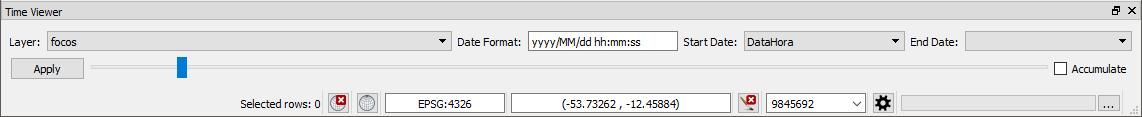
\includegraphics[width=.9\textwidth]{timeviewer-dock.png}
\caption{TimeViewer extension deployed screen}
\label{fig:timeViewerDock}
\end{figure}

\section{Results}

To validate the implementation, tests were done using some time samples obtained through the databases previously mentioned. Two types of sample data were selected, where the first one has samples with data of fire outbreaks throughout the region of Brazil, each focus has a unique date and time attribute, being necessary that the user defines this date format through graphical interface and select the table attribute that matches the date in the initial date field, ignoring the final date field as Figure~\ref{fig:timeViewerData1}.

\begin{figure}[ht]
\centering
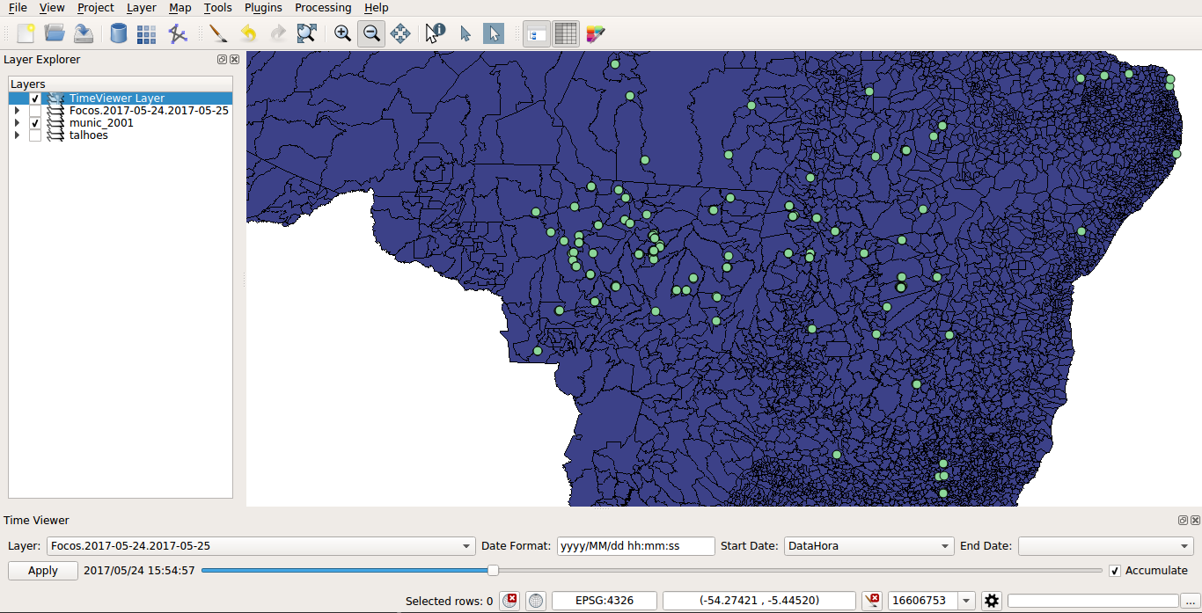
\includegraphics[width=.6\textwidth]{timeviewer-data1.png}
\caption{Using TimeViewer to view sample data from fire outbreaks}
\label{fig:timeViewerData1}
\end{figure}

The second example data has samples with data from fields in the Cabo Verde region in the state of Mato Grosso, where each plot has two date attributes, which are the starting date and end date, the user must define the date format through the graphical interface and select the table attribute that matches the start date and attribute that corresponds to the end date, as Figure~\ref{fig:timeViewerData2}.

\begin{figure}[ht]
\centering
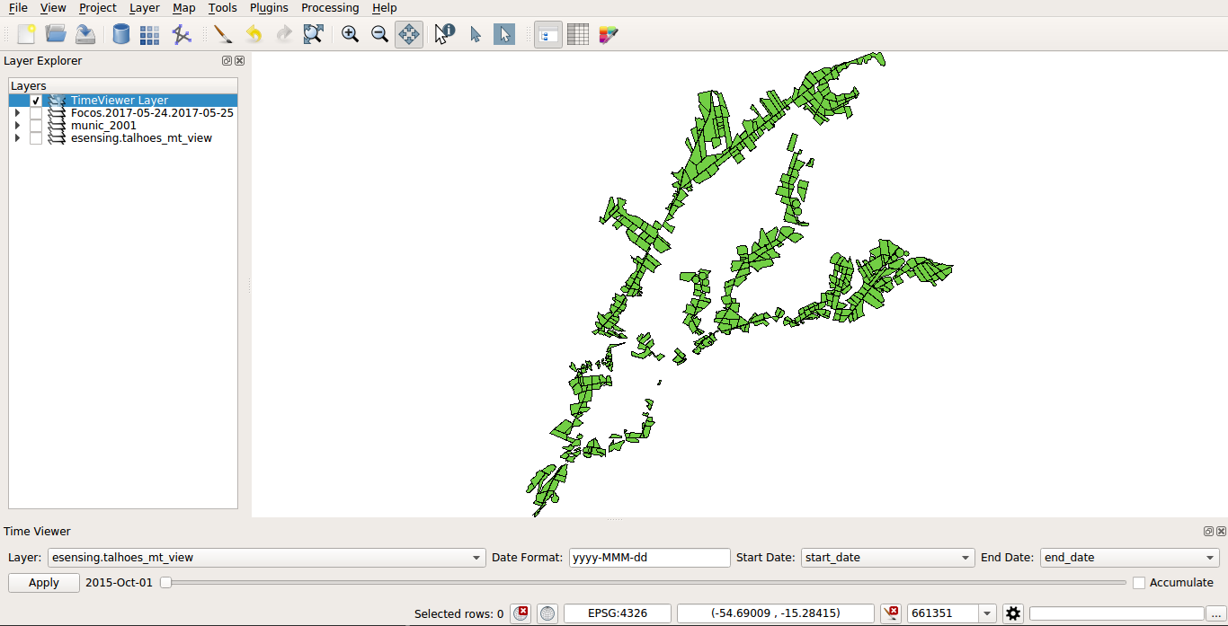
\includegraphics[width=.6\textwidth]{timeviewer-data2.png}
\caption{Using TimeViewer to view plots in Cabo Verde (MT)}
\label{fig:timeViewerData2}
\end{figure}

\section{Conclusion and Future Works}

As we can notice the amount of geographic data with temporal characteristics tends to grow constantly generating a large dataset (Big Data), with this it is difficult to use this type of data in GIS, since there is not a complete standard for visualize and manipulate temporal data. This is a problem that can be avoided through initiatives such as the proposal made by this and other works. The tool developed sought to facilitate the visualization of temporal data in a simple way, so that a non-technical user can visualize their data in the most simple and intuitive way possible.

The objectives of this work were achieved and with this new ideas were designed so that the tool can help users with new features such as, allow the monitoring of a single object and its timeline, allow the creation of an animation that can be executed in the TerraView and saved on the user's machine, use the application's own captioning tool to facilitate the visualization of changes that occur in time for attributes of samples with fixed locations in space and integration with TerraLib's Spatio Temporal module that can provides a more accurate view of temporal data types allowing their manipulation.

\bibliographystyle{sbc}
\bibliography{sbc-template}

\end{document}